\documentclass[a4paper,12pt]{report}
\usepackage{fancyhdr}
\pagestyle{fancy}
\usepackage{amsfonts}
\usepackage{amsmath}
\usepackage{tikz}
\usepackage[utf8]{inputenc}
\usepackage[serbianc]{babel}
\usepackage{titling}
\usepackage{caption}
\usepackage{subcaption}
\usepackage{titlesec}
\usepackage{fancyhdr}
\usepackage[bookmarks]{hyperref}
\usepackage{graphicx}
\graphicspath{ {images/} }

\usepackage[margin=2.5cm]{geometry}
\addtolength{\hoffset}{0.5cm}
\addtolength{\textwidth}{-0.5cm}

\fancyheadoffset{1 cm}

\setlength\parindent{0pt}

\titleformat
{\chapter} % command
[display] % shape
{\bfseries\Large\itshape} % format
{Glava \ \thechapter} % label
{0.5ex} % sep
{
    \rule{\textwidth}{1pt}
    \vspace{1ex}
    \centering
} % before-code
[
\vspace{-0.5ex}%
\rule{\textwidth}{0.3pt}
] % after-code

\pagestyle{fancy}
\fancyhf{}
\rhead{Glava \ \thechapter}
\lhead{\thesection}
\cfoot{\thepage}

\captionsetup[figure]{name=Slika}


\begin{document}
\renewcommand*\contentsname{ }

\begin{titlepage}
\begin{center}

	\textbf{\Large Univerzitet u Beogradu}\\[0.5cm]
	
	{\large Matematički fakultet}\\[6cm]
	
	\textsc{\small Seminarski rad u okviru kursa\\Uvod u bioinformatiku}\\[0.5cm]
	
	
	\textbf{\Large Poređenje sekvenci velikih razmera}\\[10cm]

	\begin{tabular}{|l|l|}
  		\hline
	    Studenti: & Annamaria Piri \\ \cline{2-2}
	              & Ozren Demonja \\ \hline
	    Školska godina: & 2016/2017. \\ \hline
	    Profesor: & Dr Jovana Kovačević	 \\ \hline
	    Datum &  28.05.2017 \\ \hline
	\end{tabular}

\newpage
\end{center}
\end{titlepage}

%\begin{center}
%	\textbf{\large SADRŽAJ}
%\end{center}
%\tableofcontents 
%\newpage

\chapter{Uvod}

Kako tehnika sekvencioniranja neprestano napreduje i biva sve jeftinija, broj sekvenci koje se dodaju u biološke baze raste eksponencijalno.  Za dati skup povezanih bioloških sekvenci prvi i najvažniji korak je njihovo poređenje. Poređenje dve ili više sekvenci se radi uz pomoć procedure poravnanja sekvenci. Ova procedura se odnosi na međusobno istraživanje stepena sličnosti sekvenci, njihovih obrazaca konzervacije i evolucione veze koje međusobno dele.

\subsection{Homologija, sličnost I identitet:}
Kada govorimo o dve sekvence obično nas zanima kakvi odnosi važe između njih. Izrazi homologija i sličnost se često koriste kao sinonimi, ali ova dva termina predstavljaju različite odnose. Homologija je kvalitativni termin koji se koristi da opiše zajedničko evoluciono poreklo pri tome ne navodeći koliki je zaista nivo srodnosti. Homologne sekvence mogu se opisati bilo kao ortologe ili paraloge. Ortologi su one sekvence koje su prisutne u različitim vrstama i imaju isto poreklo dok su paraloge sekvence koje su prisutne u isim vrstama i pojavile su se zbog dupliranja gena. Da bi opisali povezanost kvantitativno koristimo identifikaciju i sličnost. Identifikacija se odnosi na to da li su dve sekvence (ili delovi sekvence) evolucione invarijante, dok sličnost potvrđuje zamenu koja čuva strukturne ili funkcionalne uloge. Sličnost između dve sekvence je rezultat koji odražava kako identitet i supsitucija uključuju slične bazne/amino kiseline.


\subsection{Supstitucija i Homologe sekvence}
Da bi procenili sličnosti ili identičnosti koju neke dve sekvence dele potrebno je da sekvence budu poravnate. Poravnanje dve sekvence se naziva parovi poravnanja i može da se korisit za računanje sličnosti bazirano na pogotcima, promašajima ili prazninama. Mutacije koje se akumuliraju u nizu tokom evolucije su supstitucija, insercija i delecija. Supstitucija je rezultat promene u nukleotidu ili amino kiselini. Insercija i delecija (poznati zajedno kao homologe sekvence) označavaju dodavanje ili uklanjanje ostataka tipično predstavljeno crticom. Niz od jedne ili više homologe sekvence je poznatiji kao praznina u poravnanju i on se obično dosta kaznjava. Najkorišćeniji metod za računanje kazni kod praznina je kazna afine praznine.  Ovaj metod radi tako što u rezultat praznine saberemo cenu pojavljivanja praznina i pomnožimo koliko puta se pojavilo praznina za redom sa cenom pojavljivanja vezanih praznina. Ovo znači ako imamo prazninu dužine n u poravnanju, G cena pojavljivanja praznine i L cena ponavljanja praznine onda je ukupna cena jednaka G + L*n. Tipične vrednosti za pojavljivanje praznine je između 10-15 a ponavljanje 1-2. 

Drugi metod za za računanje kazni kod praznina je linearna kazna praznine. Ovaj metod je sličan kao prethodni samo što nema posebnu cenu za prvo pojavljivanje a posebnu za ponavljanje već ima samo jednu cenu.
 
U parovima poravnanja proteina, neki poravnati ostatci mogu biti slični ali ne identični. Ovi slični ostatci su označeni sa „+“ u poravnanju i nazivaju se konzervativne supstitucije.

%\chapter{Slučajevi upotrebe}


\chapter{Materijali}

\subsection{Biranje sekvenci: Dnk ili protein}
Poređenje dve sekvence se može raditi na nivou nukleotida ili na nivou proteina. Poređenje na nivou proteina može pomoći u otkrivanju važnih bioloških informacija. Takođe, mnoge mutacije u DNK se ne odražavaju na nivou proteina i ne dovode do bilo kakve promene u odgovarajućoj amino kiselini. Shodno tome, za daleke odnose između organizama sa malom identičnošću sekvence na nivou DNK, poređenje proteina je bolje.


\subsection{Poređenje parova i matrica skora}
Postoje različiti metodi koji se koriste za poravnanje. Ovi metodi uključuju analizu dot matrica, korišćenje dinamičkog programiranja i heruistički pristup.

\begin{enumerate}
\item Analiza dot matrice: Ovo je jedan od najpopularnijih grafičkih metoda za poravnanje sekvenci. Sekvence se stavljaju na X I Y osu matrice, a zatim se prolazi kroz matricu i dodaje tačka svaki put kada se naiđe na podudaranje između sekvenci. Na ovaj način tačke koje se nalaze grupisane na dijagonali signaliziraju poravnanje, dok one koje su izolovane ukazuju na slučajna poklapanja. Ovo nam lako otkriva pristup homologe sekvence i ponavljanja. Mana dot matrica je što nam daju samo grafičku reprezentaciju i ne otkrivaju nam koliko su zaista slične sekvence.
\end{enumerate} \vspace{5mm}

Zbog gore pomenute mane dot matrica drugi metodi su razvijeni za bodovanje svakog para poravnate sekvence. Jedan od takvih metoda je zasnovan na dinamičkom programiranju. Optimalno poravnanje dve sekvence se dobija razbijanjem poravnanja na manje delove i onda spajanje ovih malih poravnanja u maniru sekvence. Dinamičko programiranje identifikuje poravnanje sa najvećim skorom. Podatci se čuvaju u matricama 20x20 za amino kiseline i 4x4 za nukleotide. Ove matrice služe kao evolutivni model i koriste se za računanje zamene jedne u odnosu na drugu amino kiselinu. Brojne matrice skora su dostupne i njihov odabir je važan jer on utiče na dobijeni rezultat.

\subsection{PAM MATRICA}
Margaret Dayhoff je predložila matrice zasnovane na zameni obrazca u grupi proteina. Dayhoff i kolege su uporedili sekvence blisko povezanih proteina u porodicama koje dele više od 85\% sličnosti. Na osnovu dobijenih rezultaka konstruisali su tabelu koja ukazuje na učestalost zamene amino kiseline na jednoj poziciji kojom je definisana relativna mutacija amino kiseline. Kako su proteinske sekvence koje su korišćene vrlo blisko povezane, bilo je očekivano da posmatrane mutacije neće uticati na funkciju proteina. Ove matrice se nazivaju PAM matrice.

Zamena jedne amino kiselike drugom sa sličnim biohemiskim osobinama je ponekad prihvatljivo u proteinu. Ove zamene su poznate kao konzervatine zamene. Na primer zamena serina sa treoninom. Manje prihvatljive su one zamene koje imaju neku strukturunu ili funkcionalnu ulogu proteina i njihova zamena može imati štetne efekte. 

Dayhoff i kolege su definisale matricu PAM1 koja proizvodi 1 dozvoljenu mutaciju na 100 amino kiselinskih ostataka. Po konvenciji PAM0 je matrica identiteta (nema dozvoljenih mutacija).  Pošto je PAM1 zasnovana na blisko povezanim proteinskim sekvencama koje imaju više od 85\% identiteta sekvence, njegova upotreba je ograničena. Zato postoje druge vrste PAM matrica izvedene iz PAM1 matirce množenjem matrice sa samom sobom. Recimo PAM250 matrica znači da se PAM1 mnozi 250 puta sama sa sobom i onda se koristi za proteine koji dele 20% sličnosti sekvence. 

Izbor PAM matrice zavisi od srodnosti proteinske sekvence. Ako je sekvenca blisko povezana koristi se niža vrednost PAM matrice i obrnuto. Problem sa PAM matricama je što su zasnovane na malom broju proteinskih sekvenci dostupnih 1978. Sa povećanjem broja sekvenci potrebno je ažuriranje PAM matrica. Takodje ova matrica podrazumeva da svako mesto ima istu mutabilnost. Uprkos svim ovim ograničenjima ove matrice su i danas u upotrebi. 


\subsection{BLOSUM}
Koristeći nešto drugačiji pristup S. Henikoff I J.G. Henikoff su osmislili drugačiji tip bodovanja matrica koji opisuju nedostatke u PAM matrici. Pristup je zasnovan na korišćenju BLOCKS baze podataka koja se sastoji od velikog broja višestrukih lokalnih poravnanja daleko povezanih proteina. Glavni cilj je bio da se zameni PAM matrica pomoću mnogo većeg skupa podataka. Blokovi predstavljaju poravnanja bez praznina. Henikoff-i su ispitali oko 2000 blokova koji predstavljau više od 500 grupa povezanih proteina. Zamenili su one grupe proteina koje imaju sličnost višu od praga kod jednog predstavnika ili prosečne težine. Prag do 62\% (BLOSUM62) se najčešće korisit i on predstavlja podrazumevanu matricu skora za BLAST pretragu.

U BLOSUM matrice su time direktno izračunate evolucione razdaljine i bazirane su na očuvanju regije. Ovo čini BLOSUM matrice osetljivije samim tim i pogodnije od PAM matrica za lokalna poravnanja. Kao i kod PAM matrice BLOSUM predstavlja broj koji označava stepen konzervacije proteina sekvence koje su korišćenje za izvođenje tog konkretnog BLOSUM-a.


\section{Globalno i Lokalno poravnanje}
U ovom poglavlju posmatramo vrste poravnanja i algoritme koji upravljaju ovim poravnanjima. Postoje dva glavna tipa poravnanja: lokalna i globalna. Globalna poravnanja su ona poravnanja koja se poravnavaju celom svojom dužinom. Ovo znači da oba kraja svake sekvence učestvuju u usklađivanju bez obzira na pogotke, promašaje i praznine, sto povlači dosta praznina pa je preporučljivo da se korisit kod sekvenci približno iste dužine i visoke sličnosti. Nekad se dešava da sekvence mogu biti slične samo u nekim regionima. Ako je ovo slučaj globalno poravnanje ovako definisano može preskočiti te regione, pa zbog toga uvodimo lokalno poravnanje. Lokalno poravnanje pretraga traži regione visoke sličnosti bez obzira na dužinu sekvence.


\subsection{Needleman i Wunsch Algoritam: Globalno poravnanje sekvenci}
Saul Needleman i Christian Wunsch su 1970 predstavili jedan od važnijih algoritama za usklađivanje dve sekvence proteina. Ovaj algoritam su kasnije poboljšali Seller i Gotoh. Algoritam teži da proizvede optimalna poravnanja dve sekvence tako što uvodi praznine. Algoritam se sastoji od 3 koraka: 

\begin{enumerate}
\item Pravljenje matrice:  Dve sekvence se postavljaju u matricu prva vertiklano (po Y osi), druga horizontalno (po X osi). Ako su sekvence identične na dijagonali matrice će se naći idealno poravnanje počevši od donjeg desnog ugla idući ka gornjem levom. Praznine su predstavljene horizontalnom ili vertikalnom ivicom.
\item Ocenjivanje matrice: Neka imamo dve sekvence dužina a i b. Matrica skora će biti dimenzija a+1 x b+1. U levi gornji ugao matrice dodajemo vrednost 0. Zatim u prvu kolonu i prvu vrstu matrice dodajemo vrednosti kazne za prazninu. Kada smo popunili prvu vrstu i prvu kolonu popunjavamo ostatak matrice. Za svaku ćeliju u matrici vrednost je maksimum vrednosti iz ćelije dijagonalno iznad („+/-“ pogodak/promašaj), ćelije direktno iznad („-“ kazna za poravnanje) i ćelije levo („-“ kazna za poravnanje).   
\item Identifikovanje optimalnog poravnanja: Kada smo popunili matricu trebamo odrediti optimalno poravnanje. Najlakši način je proces praćenja unazad. Krenemo od donjeg desnog ugla i određujemo iz koje ćelije se dobio naš rezultat. Zatim uzimamo tu ćeliju i ponavljamo postupak. Put koji dobijemo odgovara optimalnom poravnanju. Nekad možemo dobiti da je rezultat došao iz dve ili tri ćelije i onda dobijamo višestruka optimalna poravnanja. Dalje nastavljamo tako što vršimo praćenje unazad iz svake od tih ćelija.  

\end{enumerate} \vspace{5mm}

\subsection{Smith i Waterman Algoritam: Lokalno poravnanje sekvenci}
Smith i Waterman algoritam se koristi da nađe regione lokalne sličnost i teži da poravna samo delove dve sekvence bez uvođenja praznina. Konstrukcija matrice je slična kao i kod Needleman i Wunsch algoritma, ali se sistemi za ocenjivanje matrice malo razlikuju.  Algoritam se sastoji od tri koraka:

\begin{enumerate}
\item Pravljenje matrice: Isti kao i kod Needleman i Wunsch algoritma.
\item 2. Ocenjivanje matrice: Neka imamo dve sekvence dužina a i b. Matrica skora će biti dimenzija a+1 x b+1. U prvu kolonu i prvu vrstu matrice dodajemo vrednosti 0. Zatim kao i kod globalnog poravnanja, za svaku ćeliju u matrici vrednost je maksimum vrednosti iz ćelije dijagonalno iznad („+/-“ pogodak/promašaj), ćelije direktno iznad („-“ kazna za poravnanje) i čelije levo („-“ kazna za poravnanje). Ali za razliku od globalnog ako je maksimum negativan stavljamo 0 u ćeliju.   
\item Identifikovanje optimalnog poravnanja: Kada smo popunili matricu trebamo odrediti optimalno poravnanje. Najlakši način i ovde je proces praćenja unazad. Počinjemo od najveće vrednosti u matrici, a zatim je procedura ista kao i kod globalnog poravnanja samo što se ne zaustavljamo u gornjem levom uglu nego kad dođemo do 0. Ova ćelija označava početak poravnanja.  

\end{enumerate} \vspace{5mm}

Ova dva algoritma nalaze optimalno poravnanje ili poravnanja ali su poprilično spora.  Ako imamo dve sekvence dužine a i b složenost je O(axb). Ovo je neefikasno kada poredimo neke sekvence sa sa celom bazom. Zato se danas koriste heruistički pristupi. Glavni algoritmi koji upotrebaljavaju heruistički pristup su FASTA I BLAST. Oni su bazirani na lokalnom poravnanju ali rade značajno brže. U sledećem poglavlju opisujemo ove algoritme.
\newpage

\chapter{Metodi}

\subsection{BLAST}
Poređenje dve sekvence može se raditi na nivou nukleotida ili na nivou proteina. Poređenje na nivou proteina može pomoći u otkrivanju važnih bioloških informacija. Takođe, mnoge mutacije u DNK se ne odražavaju na nivou proteina i ne dovode do bilo kakve promene u odgovarajućoj amino kiselini. Shodno tome, za daleke odnose između organizama sa malom identičnošću sekvence na nivou DNK, poređenje proteina je bolje.


\subsection{Objašnjenje}
BLAST je skraćenica od Basic Local Alignment Search Tool koji su dizajnirali Eugene Myers, Stephen Altschul, Warren Gish, David J. Lipman i Webb Miler. Kao što samo ime kaže zasniva se na lokalnom poravnanju niski proteina ili amino kiselina. BLAST je značajno brži od običnog Smith-Waterman algoritma i od FASTA metoda (kasnije naveden). Heurističkim algoritmima upoređuje datu nisku sa bazama. Ne ocenjuje poklapanje i neslaganje univerzalno, nego po nekim statistikama izračuna značajnost konkretnih slaganja/neslaganja i pomoću njih izračunava ukupnu ocenu. Na osnovu toga kako su zadati ulazni podaci i kakvu bazu potražujemo, BLAST metode možemo da kategorišemo u pet potkategorija:
\begin{enumerate}
\item Nukleotid BLAST: DNK nisku uporedi sa DNK bazom podataka
\item Protein BLAST: nisku proteina uporedi sa proteinskom bazom podataka
\item Blastx: datu DNK sekvencu prevodi na šest mogućih načina u nisku proteina i to uporedi sa proteinskom bazom podataka
\item Tblastn: datu sekvencu proteina uporedi sa DNK bazom podataka, tako da DNK niske iz baze prevede u nisku  proteina
\item Tblastx: i zadatu DNK nisku i DNK niske prevede prvo u niske proteina pa posle ih upoređuje
\end{enumerate} \vspace{5mm}

Prilikom korišćenja algoritma koristimo neke bitne parametre:

\begin{enumerate}
\item Očekivan prag: (E-value odn. E-vrednost) predstavlja očekivan broj slučajnih pogodaka kod traženja u bazi. Za BLAST je E-vrednost obično 10.
\item Veličina reči: (k) algoritam je osnovan na k-merima. Obično  se kod proteina koriste 3-meri (kod manjih peptida nekad 2-meri) a kod aminokiselina 11-meri (vrednost može da varira između 7 i 15). Što kraće k-mere koristimo to precizniji rezultat dobijemo ali gubimo na vremenu potrebnom za pretragu baze podataka.
\item Matrica skora: Kada su niske aminokiselina u pitanju, izborom nekog od pre opisanih matrica PAM ili BLOSUM (u zavisnosti od prirode problema) ocenjujemo pogodke, pomašaje i praznine. Kod niske nukleotida obično pogodak (match) se boduje sa "+1", promašaj (mismatch) "-2" a praznine linearno, bez kažnjavanja ulazka u prazninu.
\item Prag T: prag se odnosi na skor kod traženja poravnanja prvog k-mera. Što veći T to precizniji rezultat, ali može da previdi neke moguće k-mere.
\end{enumerate} \vspace{5mm}

BLAST algoritam prvo podeli niske na k-mere, pa prilikom traženja nađe ne samo one niske koje se preklapaju slovo po slovo, nego i one koje sadrže neki promašaj slova. 
U sledećem primeru VLD poravnamo sa VLE. Pogledamo sve 3-mere od kojih najveći skor ima KYN sa KYN. Proširimo poravnanje levo i desno.

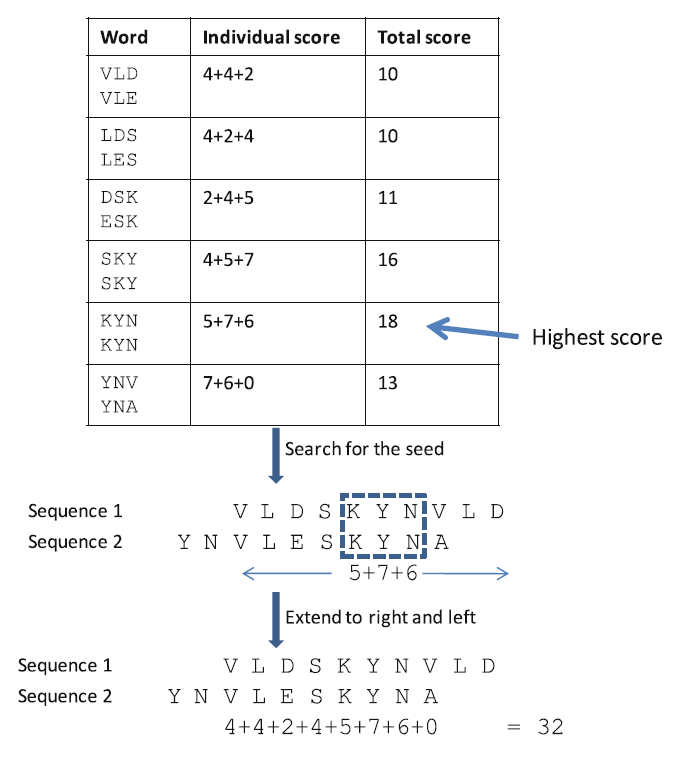
\includegraphics{blast}

\subsection{PSI-BLAST}
Vrsta BLAST metode za traženje proteina koji su slični ali u manjoj meri. Specifičnost ove varijante metoda je da matrica skora zavisi od pozicije u niski.

\subsection{PHI-BLAST}
Specializovan BLAST koji omogućava traženje šeme u bazi podataka. Na primer jedno parče aminokiseline koje je korisno kod identifikacije proteinske porodice.

\section{FASTA}
Slično kao BLAST, radi sa k-merima (obično 1-2 kod proteina i 4-6 kod nukleotida) i traži pogodke koji su blizu, povezuje ih ali bez uvođenja praznina, i na osnovu povezanih regija izračuna neku inicijalnu ocenu. U sledećem koraku program izabere 10 najboljih regija i sa običnim Smith-Waterman algoritmom traži poravnanje u parovima.

\subsection{Metode i alate}

\subsection{MegaBLAST}
Program kod NCBI koji je prilagođen traženju jako sličnih DNK seknvence. Brži je od običnog BLAST-a zato što veličina reči kod uparivanja je visoka, obično 28 a u nekim slučajevima je čak 64 karaktera. Druga specifičnost koji utiče na brzinu je da praznine kažnjava na uniformalan način. (nema razlike kod otvaranja praznine)

\subsection{BLAT}
Program je napravljen za poravnanje dugačkih DNK niski sa minimum 95% poklapanjem za vrlo brzo vreme.

\subsection{BLATZ}
Program traži ponovjene regije u prvom genomu, koje su prisutne i u dugom genomu. Briše ove regije. Posle traži niske od 19 nukleotida od kojih je minimum 12 pogodaka u poravnanju. Ove niske nastavi da proširi bez praznine dok ocena poravnanja ne preskoči neki definisan prag.

\subsection{LAGAN}
Veoma efikasan alat za poravnanje dve niske. Prvo potraži jedno optimalno lokalno poravnanje, koji služi kao temelj daljeg algoritma CHAOS. CHAOS traži kratke niske koje se ne moraju slovo po slovo preklapati. Na osnovu prethodnih generiše jednu grubu globalnu mapu, pa na kraju finalno poravnanje.

\subsection{MUMMER}
Alat koji radi lokalno poravnanje pomoću sufiksnih stabala. Poznat je po tome da nalazi sve posebne podniske sa velikom efikasnošću i među njima izabere maksimalne jedinstvene takozvane MUM-ove (Maximal Unique Match). U sledećem koraku izdvoji najduže koji pripadaju u oba genoma a regije među njima poravna Smith-Waterman algoritmom.

\subsection{Mugsy}
Jedan od alata koji poravna više genoma u isto vreme. Koristi se za traženje duplikacija ili delova gde se desilo premeštanje u genomu.

\subsection{WABA}
Program se koristi kad je u pitanju poravnanje dugačkih niski. Traži niske od 6 karaktera, na osnovu šeme 11011011 nađe inicijalne pogotke, gde 1 mora da bude pogodak(match). Ovako efikasno radi sa indelima. (insertion i deletion)

%\newpage

%\input{./grafika_slucajevi.tex}
%\newpage

%\input{./zakljucak.tex}


\end{document}
